\documentclass{article}
\title{CSC301 HW9}
\author{Alex Zhang}
\date{April 2023}
\textwidth=16.00cm 
\textheight=22.00cm 
\topmargin=0.00cm
\oddsidemargin=0.00cm 
\evensidemargin=0.00cm 
\headheight=0cm 
\headsep=0.5cm
\textheight=610pt
\usepackage{graphicx}



\graphicspath{ {./images/} }

\usepackage{latexsym,array,delarray,amsthm,amssymb,epsfig}
\usepackage{amsmath}
\usepackage{listings}
\lstset{
  basicstyle=\ttfamily,
  mathescape
}


\newcommand{\bmat}[1]{\begin{bmatrix} #1 \end{bmatrix}}
\newcommand{\mat}[1]{\mathbf{#1}}

\let\ds\displaystyle

\begin{document}
\maketitle

\section*{Question 1}

\section*{Question 2}
Based on the recurrence, I can draw the following recursive table:
\begin{center}
    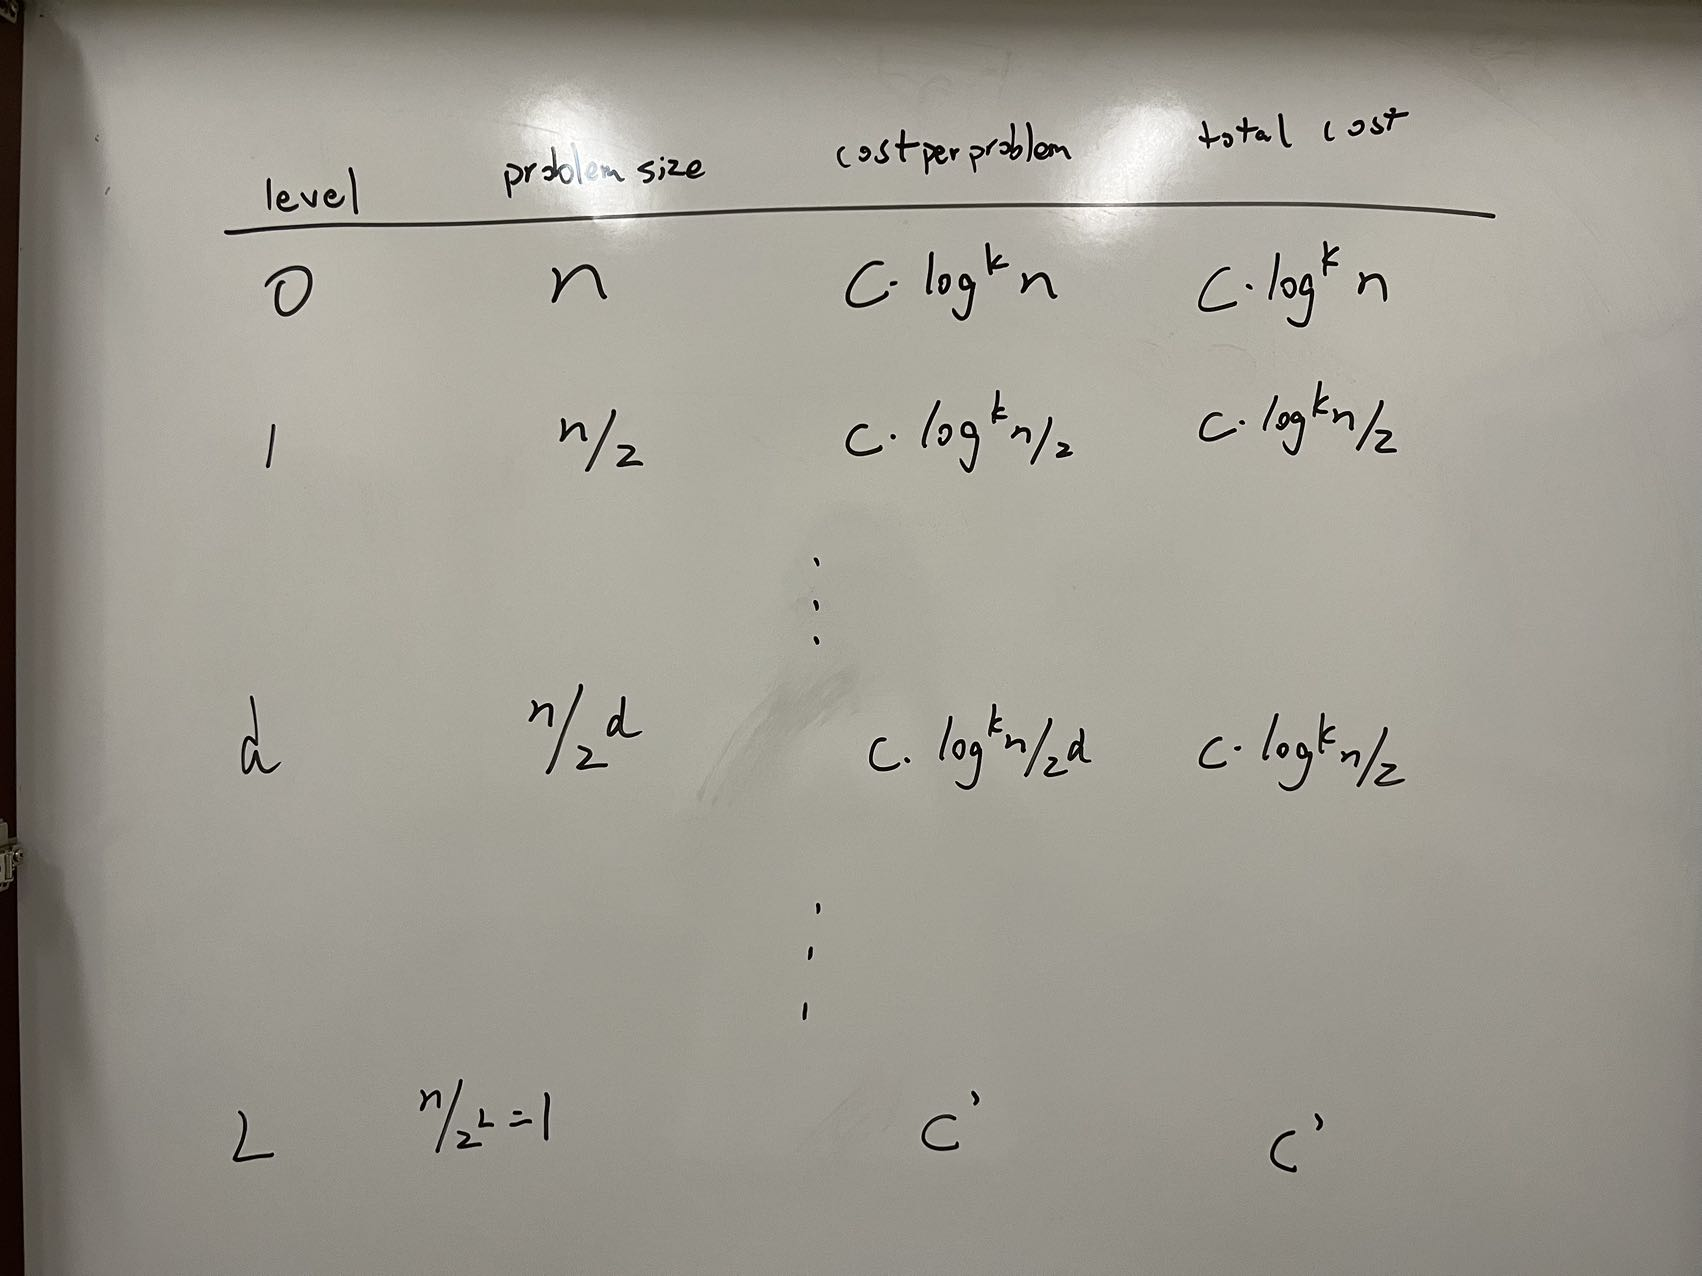
\includegraphics[scale = 0.15]{cool.jpg}
\end{center}
From this table, since there are total $L+1$ levels and $L = \log_2 n$, 
the total work will be, 
$$c \cdot \sum^{\log_2 n -1}_{d=0}\log^k (n/2^d) + c^\prime $$
doing transformation for each addition part,
$$c \cdot \sum^{\log_2 n -1}_{d=0}(\log_2 n - \log_2 2^d)^k + c^\prime $$
\paragraph{Case 1:} Big-Oh \\
Since $\log_2 2^d = d$ and $d \geq 0$, $(\log_2 n - \log_2 2^d)^k$ will always smaller than $\log^k_2 n$.
This shows that 
\begin{align}
    c \cdot \sum^{\log_2 n -1}_{d=0}(\log_2 n - \log_2 2^d)^k + c^\prime &\leq c \cdot \sum^{\log_2 n -1}_{d=0}(\log_2 n)^k + c^\prime \\ \nonumber
    c \cdot \sum^{\log_2 n -1}_{d=0}\log^k (n/2^d) + c^\prime &\leq c \cdot \sum^{\log_2 n -1}_{d=0}(\log_2 n)^k + c^\prime \\ \nonumber
    &= c \cdot \log_2 n \cdot (\log_2 n)^k + c^\prime \\ \nonumber
    &= c \cdot \log^{k+1}_2 n + c^\prime \nonumber
\end{align}
Because $c$ and $c^\prime$ are both constant, let $g(n) =\log^{k+1}_2 n $, $f(n) =\sum^{\log_2 n -1}_{d=0}\log^k (n/2^d) + c^\prime$, if $c \textmd{,} N> 0$
$$f(n) \leq c \cdot g(n)$$
for all $n \geq N$, then 
$$f(n) = O(g(n)) = O(\log^{k+1}_2 n)$$

\paragraph{Case 2:} Big-Omega\\
Generally speaking, the following inequality,
$$  \frac{\sum^{\log_2 n -1}_{d=0}\log_2^k (n/2^d)}{10} \leq  \sum^{\log_2 n -1}_{d=0}\log_2^k (n/2^d)$$
holds true.









\section*{Question 3}




\end{document}